\documentclass[conference]{IEEEtran}
\IEEEoverridecommandlockouts
% The preceding line is only needed to identify funding in the first footnote. If that is unneeded, please comment it out.

\usepackage[utf8]{inputenc}
\usepackage[english]{babel}
\usepackage{fancyhdr}
\usepackage{lastpage}
\usepackage{float}
\usepackage[table]{xcolor}
\usepackage{url}

\pagestyle{fancy}
\fancyhf{}

\rfoot{Page \thepage \hspace{1pt} of \pageref{LastPage}}


\usepackage{cite}
\usepackage{amsmath,amssymb,amsfonts}
\usepackage{algorithmic}
\usepackage{graphicx}
\usepackage{textcomp}
\usepackage{xcolor}
\def\BibTeX{{\rm B\kern-.05em{\sc i\kern-.025em b}\kern-.08em
    T\kern-.1667em\lower.7ex\hbox{E}\kern-.125emX}}
\begin{document}

\title{Comparing 3D Rendering Engines in Blender}

\author{\IEEEauthorblockN{Lovász Ákos}
\IEEEauthorblockA{\textit{Eszterházy Károly University} \\
\textit{Computer Science BSc}\\
Eger, Hungary \\
akos4x44@gmail.com}
\and
\IEEEauthorblockN{Dombi Tibor}
\IEEEauthorblockA{\textit{Eszterházy Károly University} \\
\textit{Computer Science BSc}\\
Eger, Hungary \\
dombidav@gmail.com}
}

\maketitle

\tableofcontents


\begin{abstract}
Using most 3D modeling and/or animation software, there are multiple choices for visualization. As Computer Graphics have evolved over the years, there has been an increased demand for computer generated visuals in use of movies, advertisements, product designs and so much more. Render engines are an essential part of turning project ideas into real products and different engines can produce different results. This raises the question: "What render engine is right for me?". In this paper we compare 3 of the easiest and most accessible engines withing Blender: Cycles, LuxCore and EEVEE, showing the differences between the subjective and objective differences of the end products, while monitoring hardware usage and measuring render times to conclude what render engine could be the most optimal choice for a given scene.
\end{abstract}


\section{Introduction}
With the rapid evolution of the computer graphics market, countless dedicated software appears each year, aiming to satisfy every need of the designers. With millions of downloads every year, one of the most popular is Blender, an open-source, cross-platform 3D creation suite. Although Blender is free, it is a competitive alternative to commercially available 3D design software and is also one of the most comprehensive editor suites on the market. Nowadays Blender is used in numerous professional industries, such as video game development, film making, product design and the list goes on.
The last step of the production pipeline is rendering. This is the process of creating the actual 2D image (or animation, but we are not covering that) from the prepared scene. This can be compared to taking a photo or filming a scene in real life. Over the years, several different methods have been developed. When we render our scene, we can choose our rendering engine consequently choosing our method to visualize our scene.
In this paper, we will compare the 3 most popular, and most accessible rendering engines for Blender, which are the following:

\subsection{Cycles} \label{cycles_section}

Cycles is a physically-based direct light sampling path tracer included with Blender since 2011, version 2.61. It is designed for production rendering, it supports multi-core CPU rendering and Multi-GPU rendering too. For GPU render Cycles uses the NVIDIA CUDA or AMD OpenCL technology.
Cycles is relatively easy to set up and fine-tune which makes it a good choice for beginners.\cite{blenderCyclesIntro} However, it's flexible shading nodes, subdivision handling and built-in denoiser can satisfy most of the production needs. This engine is under the Apache License v2,\cite{cyclesFeatures} therefore, we can use it in commercial projects without concern for royalties.\cite{apacheLicense}


Despite all it's achievements, it is not a perfect engine. It struggles particularly with caustics, which are light rays reflected or refracted by curved surfaces or objects, or created by ray projection. 

\begin{figure}
\centerline{\includegraphics[scale=0.6]{Images/caustics.jpg}}
\caption{Caustics projected onto a surface by a glass object}
\label{causticsIRL}
\end{figure}

This is because cycles creates images by casting rays from the camera, bouncing it in the scene, until they hit a light-emitting object or leaves the scene completely. If a ray has not reached a light source after a pre-determined number of bounces, it is terminated. This limit can be configured by the user, it's not a hard coded number. Changing this value can have massive impacts on performance and in many cases altering the value of the permitted bounces can fix visual errors or simply increase performance. To find a light source, bidirectional scattering distribution function, or BSDF is used.\\\\

\begin{figure}[htbp] % Nem tudom mi az a `hbt!` de anélkül az oldal tetejére rakja a képet
\centerline{\includegraphics[scale=0.4]{Images/PathTracing.png}}
\caption{Path of a light ray in unidirectional path-trace}
\label{PathTracing}
\end{figure}

There are two separate types of integrators in cycles.
\begin{itemize}
    \item The default path tracing, which is a pure path tracer. It casts rays from the camera and treats these rays as photons. These rays can hit objects, light sources or the world background. If the ray hits an object, it bounces off the geometry and will continue until it reaches the pre-determined maximum number of bounces and it's terminated, or reaches a light source. The pixels of the result image are calculated based on multiple rays, a process knows as sampling. The sampling is also determined by the user and is the biggest factor in render times. Simply put, the higher amount of samples we use, the clearer the image gets, but will take exponentially longer to create.\\
    \item Branched path tracing is based on the default path tracer, but it takes more than one light into account when sampling. Using this method will create clearer images at the cost of performance and render time. \\
\end{itemize}

\begin{figure}[htbp]
\centerline{\includegraphics[scale=0.55]{Images/CyclesRayPath.png}}
\caption{Type of Light rays in Cycles}
\label{figlightRaysCycle}
\end{figure}

In Cycles, light rays can be divided into four categories:
\begin{itemize}
\item The Camera rays are coming from the current observing camera of the scene
\item The Reflections rays are generated by a reflective surface
\item The Transmission rays are generated by light passing through a surface
\item The Shadow rays are used to track shadows\\ % What a suprise
\end{itemize}
The reflection rays can be further categorized as a diffuse, glossy, or singular ray (perfectly sharp reflection)

\subsection{LuxCore Render}\label{luxCore}

Just like Cycles, LuxCore Render is free and open-sourced physically-based rendering software under the protection of Apache License v2. The LuxCore engine uses highly optimized state of the art algorithms thus allowing it to reproduce natural phenomena which most other rendering programs can not. While Cycles only calculates a single direction for the light rays, LuxCore Render is capable of calculating it bidirectionally. LuxCore also features physically accurate representation of a wide variety of material types, like matte, glossy, metal, glass, or even car paint. LuxCore shines when it comes to lighting. We already mentioned the problem with caustic light rays in Cycles, but thanks to the bidirectional path-tracing LuxCore uses, it can generate realistic caustic projections.

\begin{figure}[htbp]
\centerline{\includegraphics[scale=0.17]{Images/lux_caustic.jpg}}
\caption{Caustics in LuxCore Render}
\label{luxCaustics}
\end{figure}

The engine supports both light emitters and environmental lights. The distribution pattern of a light source can be defined precisely with photometric data in the form of IES diagrams. Environmental lights can be simulated with an HDR image, a sun/sky system or with a distant, infinite lamp as a generic sun and sky. LuxCore also features true motion blur as object movement is described in absolute time rather than simply over the exposure time. This allows real-world control of the camera shutter time and the resulting blur strength.\cite{LuxWiki}

\subsection{EEVEE} \label{eevee_section}

EEVEE actually stands for Extra Easy Virtual Environment Engine. It was created for Blender with the intent of providing a robust, "real-time" PBR engine fully compatible with Blender's existing tool set. It's also highly compatible with the cycles render engine, since it was built to utilise the already existing shader node system used by cycles. While LuxCore and Cycles were designed for production quality renders, like highly photo realistic images or animations, EEVEE is a "real-time" render engine. This means render time of separate frames are only a few seconds. It's not truly real-time, as it has to compile shaders, reflection maps, ambient occlusion and irradiance volumes before rendering an image and compositing effects are applied at every frame, thus adding to the render time of each frame. This adds a few seconds to the render times of frames in more complex scenes but it usually doesn't add up to more than 2-5 seconds per frame, however in the viewport, it's truly real-time, as it stores these complied values in cache and doesn't re-calculate the scene at every frame. This is very useful for example when presenting a scene to a client and quick and small adjustments can be made to the layout, lighting and even materials, without waiting hours for a new render to finish.\\


EEVEE uses a technique called rasterization where the scene's geometry is projected onto a raster of pixels instead of simulating the light itself.\cite{EEVEEWorking} With the use of OpenGL 3.3, this method is very fast, however this speed comes at the cost of accuracy.

\begin{figure}[htbp]
\centerline{\includegraphics[scale=0.4]{Images/EeveeRasterize.png}}
\caption{Rasterization}
\label{eeveeRaster}
\end{figure}

The colours of the pixels are determined with shader code based on surface normals and light positioning.  To make the output more appealing to the eye, additional procedures are needed such as anti-aliasing, light-mapping, light probes, ambient occlusion, shadow blurring, etc.

\section{Methods}

\subsection{Monitoring and logging hardware usage and temperature}
    Monitoring hardware load was a crucial point in our experiment, as we would like to see the ratios between computation power, energy consumption and heat production amongst different hardware generations. It is easy to find software to monitor CPU usage and temperatures, and some of these are even capable of logging the values. However, it was remarkably difficult to find a GPU monitoring tool with logging functionality. The main reason behind this is that sensor values of Nvidia graphical cards are not accessible from direct system calls,\cite{nvapiStack} but only from APIs provided by the company and each generation has it's own API library.\cite{nvapi}
    Our choice of monitoring software was HWiNFO, which is actually a wide variety of monitoring and diagnostic tools packed in a single program. For this reason, it supports a wide variety of hardware (including Nvidia GPUs) and it is able to monitor thermal data (CPU, GPU, Motherboard), load percentage (CPU, GPU), memory usage (RAM, VRAM), power consumption (CPU, GPU), and much more. For logging the data we used the built-in logging functionality, which saves the values of selected sensors over a period of time. \cite{hwinfo} To sort and visualize the gathered data we used Google Sheets. 
   
    

\subsection{Demo files}\label{Demo}
    During our testing, we used two example scenes, provided on the Blender.org website. The scenes we used were chosen specifically to highlight the differences between the two render engine's internal workings as well as some subjective differences between the outcomes of the final products. One of the scenes is an automotive display presentation\cite{mikeBMWscene}, which shows a combination of high-intensity direct lighting as well as an indirect, environmental light. The other scene is an architectural visualization\cite{claudio2013archviz} example, showcasing soft lighting, overlapping shadows and water reflections. 
\subsection{Hardware used}
    We were somewhat limited in the number of choices regarding hardware, but what we ended up using represents three steps of computing capacity. The CPU selection has a well-rounded range, including an older, low-spec processor and two mid-range CPUs including an "HQ" processor, that's used in portable computers. The GPU selection clearly shows the generational differences between Nvidia's 60series mid-range cards, as well as a close equivalent to the GTX 960's power one generation later, the GTX 1050Ti. We unfortunately couldn't include any representation from the AMD family of GPUs, however, as or March 2020, cycles works best with CUDA technology.\\


\begin{itemize}
    \item CPU Selection
    \begin{itemize}
        \item Intel® Core™ i5-6600
        \item Intel® Core™ i5-7300HQ
        \item AMD FX-4130\\
    \end{itemize}
\end{itemize}

\begin{itemize}
    \item GPU Selection
    \begin{itemize}
        \item Nvidia GeForce GTX 1060
        \item Nvidia GeForce GTX 1050Ti
        \item Nvidia GeForce GTX 960\\
    \end{itemize}
\end{itemize}



\subsection{Converting scenes from Cycles to LuxCore}
    Thanks to the LuxCore Project team, the engine is highly compatible with cycles for surface lever conversion, however, making scene renders look comparable takes a lot more effort than clicking the integrated "Use cycles setting" button. First off, the two engines use radically different values for light sources, so all of the emission objects require some amount of tweaking, for example the world lighting strength of the architectural visualization scene (figure \ref{fig:luxARCHvsc}) in cycles is 0.15 while in LuxCore it's 0.00001. The supported materials also differ, so there are two options when converting a scene. Allow LuxCore to interpret the cycles shading nodes and make small adjustments to the node trees to eliminate nodes that are not supported in Lux, or completely remake every material in the included LuxCore Material Node editor. Many of the shaders are very similar and share functionality, thus they can work in both engines, but for optimal results, it's recommended to use the engine's own node tree. While in our case we head to focus on scene conversion for accurate comparisons, most projects will choose their engine ahead of time so they can focus on building the best materials in the given engine rather than spending extra time before the final steps on conversion.
    
\subsection{Converting scenes from Cycles to EEVEE}
    EEVEE was built for complete Blender integration, so "converting" the scene from cycles to EEVEE is as easy as switching the engine. However there are obvious differences to the rendering approach, EEVEE being a real-time engine, some features such as reflections, volumes and ambient occlusion don't appear naturally, like in path-traced methods. In EEVEE you have to add extra objects known as "Light Probes". This category of items include reflection cubemaps for accurate pre-calculated reflections, reflection planes, which act like mirrors and irradiance volumes, that can be used to simulate fog. Adding these can enhance the scene and are necessary to make comparable renders to path-traced equivalents. Lights, textures, materials share the node tree with cycles, so there are no changes to be made on that front. Converting to EEVEE from cycles is extremely easy all thanks to the developers who always had this conversion in mind.



\section{Results}
\subsection{Hardware comparison}
As we previously mentioned our hardware choice was limited, yet we still managed to utilize three steps of hardware generations. It must be made very clear, that GPUs are vastly superior in complex computations which are needed to create realistic surfaces, light rays and reflections. While CPUs are better for a high number of simple calculations. As you can see on chart \ref{fig:rendering_time_hw_comparison}. This result is expected, as GPUs are designed for this specific task, while CPUs are only generic calculating units.

Please note that the tested AMD CPU is far behind the others because two reasons: One, the FX was arguably the least successful series of the AMD family, and two, the 4130 was made as a lower-middle-class, entry-level CPU at the time of it's release.
\begin{figure}[htbp]
        \centering
        \includegraphics[scale=0.2]{Images/renderingtimes_graph.png}
        \caption{Rendering times comparison}
        \label{fig:rendering_time_hw_comparison}
    \end{figure}

\subsubsection{CPU rendering} \label{cpu_rendering}
    As we previously stated, CPU rendering on low core-count, home configurations is strongly unadvised. Whilst there will be no difference in the final product rendering times are massively longer than GPU renders. Some industrial render farms are running CPU renders but those are not comparable to our systems in terms of computational power.
    
    So much so, that we were unable to run a full LuxCore Render on the FX-4130 as the CPU quickly overheated and automatically reduced it's performance to protect itself. Thus resulting in software instability and crashes. After this we deemed unnecessary to test LuxCore CPU render as the Intel CPUs will perform pretty similar to each other.
    
    On chart \ref{fig:rendering_time_cpu} you can see the difference between the complexity of the scenes we used and the difference in CPU generations. As expected, the much younger Intels are vastly superior. However it is worth noting, that 7300HQ is a laptop cpu and it's performance on simple scenes are pretty close to the 6600.
    \begin{figure}[htbp]
            \centering
            \includegraphics[scale=0.2]{Images/cycles_cpu_renderingtimes_graph.png}
            \caption{Rendering times comparison}
            \label{fig:rendering_time_cpu}
        \end{figure}

\subsubsection{GPU rendering the BMW scene}
    As you can see on chart \ref{fig:bmw_gpu_time} Cycles simple path-tracing method pays off in rendering time as it is three times faster on average. 
    \begin{figure}[htbp]
            \centering
            \includegraphics[scale=0.2]{Images/bmw_gpu_time.png}
            \caption{BMW rendering on GPU}
            \label{fig:bmw_gpu_time}
        \end{figure}
    
    This is mainly because LuxCore calculates massive amount of paths, reflection angles, transparency, etc. However on this scene there are very little caustic light rays, so LuxCore can not show it's full potential. Consequently there are a huge amount of the calculations are unnecessary.
    

\subsubsection{GPU rendering the ArchViz scene}
    Jumping to the much more complex ArchViz scene, we see less time difference, which progressively gets lower with each GPU generations as we see on chart \ref{fig:archviz_gpu_time}.
    
    
    \begin{figure}[htbp]
            \centering
            \includegraphics[scale=0.2]{Images/archviz_gpu_time.png}
            \caption{ArchViz rendering on GPU}
            \label{fig:archviz_gpu_time}
        \end{figure}
    On this scene we can utilize the power of LuxCore better as we see on reflections and the interior parts (figure \ref{fig:cyclesARCHvsc}).

\subsection{Hardware usage}
    During our experiments we also logged hardware usage, temperature and power consumption. First of all, rendering always uses as much resource as it is available (or as much the operating system allows). This means we always see 100\% CPU or GPU load. In some software (like Maya or 3ds Max) it is possible to limit the maximum resource usage, Blender does not provide this kind of function, however it is possible to limit how many CPU cores are used during rendering. For this reason in this section we will talk about generation advancement between graphic cards. Also note that GTX 1050Ti is operating in a Laptop, whilst the other two are in desktop configurations.
    
    \subsubsection{Testing with Cycles}
        For this test we only used the ArchViz scene as it takes much more time to render than the BMW scene, and because of this, the collected temperature data will provide more relevant information. On the following curve diagram you can follow temperature data thorough the rendering time:
        \begin{figure}[htbp]
            \centering
            \includegraphics[scale=0.3]{Images/cycles_archviz_gpu_graph.png}
            \caption{ArchViz rendering temperatures}
            \label{cycles_temp}
        \end{figure}
        As you can see GTX 960 peeks at exactly 50°C (actual maximum was 51°C for about 20 seconds) which is probably a software controlled cap value. At this temperature the card will lower it's performance to not exceed this value. However, GTX 1050Ti and 1060 can operate on a little higher temperature 57°C and 60°C respectively. It is worth noting, that the 960 and 1050Ti cooled back to their idle temperature in about 20 seconds, but 1060 only needed half of this time, which shows it's advanced cooling solution.
        
        Power consumption wise we can not compare the hardware as GTX 1050Ti, as it is in a laptop, does not provide any sensor value about it's current energy consumption. While 960 and 1060 can not be compared either, because while the i5-6600 contain an integrated GPU (HD Graphics 530) the FX-4130 does not, and we could not test out different combinations of the mentioned hardware. This means on the i5-6600 configuration, in idle state, the operating system can switch to the integrated GPU and turn off the high power consumption graphic card entirely. However it is worth noting on diagram \ref{cycles_pwr}, that while the 1060 uses minimal electricity in idle state, when it needs to calculate it uses much more power than the 960. This means 960 can operate on power units with smaller effective wattage as it was designed as a lower cost graphic card.
        \begin{figure}[htbp]
            \centering
            \includegraphics[scale=0.3]{Images/cycles_archviz_gpu_power_graph.png}
            \caption{ArchViz rendering power consumption}
            \label{cycles_pwr}
        \end{figure}

\subsection{Visual Differences}

\subsubsection{Cycles versus EEVEE render result}
    When comparing a real-time engine shown on figure \ref{fig:eeveeBMWvse} to a path tracer, shown on figure \ref{fig:cyclesBMWvse} the visual differences are obvious, given that EEVEE uses cheaper, faster, less accurate calculations to shadows and reflections to cut down on render times.
    \begin{figure}[htbp]
        \centering
        \includegraphics[scale=0.2]{Images/BMWcycles.png}
        \caption{Cycles BMW render}
        \label{fig:cyclesBMWvse}
    \end{figure}
    \begin{figure}[htbp]
        \centering
        \includegraphics[scale=0.2]{Images/BMWeevee.png}
        \caption{EEVEE BMW render}
        \label{fig:eeveeBMWvse}
    \end{figure}
    This comes at the cost of realism but it's important to mention that this is still a very competent result for some applications such as game design, quick iterative work or in kinds of environments where the importance of quick renders far outweigh realism.\\
    The most striking difference comes from the hard-edged shadows, simple, faked reflections and an overall simpler image. This is a result of EEVEE not simulating light rays unlike cycles, meaning that reflections and shadows come from simple calcualtions as opposed to simulating light scattering over multiple types of surfaces with varied levels of reflective and refractive properties.
\\
\subsubsection{LuxCore versus Cycles render result}

     
     
      \begin{figure}[htbp]
        \centering
        \includegraphics[scale=0.2]{Images/ARCHlux.jpg}
        
        \caption{LuxCore ArchViz render}
        \label{fig:cyclesARCHvsc}
    \end{figure}
     
    In this architectural visualization scene, the final renders are fairly similar between the two path tracer engines LuxCore and Cycles. The former, visible on figure \ref{fig:luxARCHvsc} handled the scene's soft, sunset lighting than the latter, shown on figure \ref{fig:cyclesARCHvsc}. The pool's reflections are more visible and sharper. 
    \\\\
    
    The indoor areas also suffer with cycles, due to it's very young denoiser leaving much more noticeable artifacts on darker areas, as opposed to LuxCore's cutting edge denoiser that's much more advanced and produces clearer images with even less information than cycles. This doesn't come without it's own problems, however. Some textures have visibly less detail as a result of over-smoothing in LuxCore's denoising algorythm, thus the cycles render retains more small-scale details on some textures.\\

    
    \begin{figure}[htbp]
        \centering
        \includegraphics[scale=0.2]{Images/ARCHcycles.jpg}
        
        \caption{Cycles ArchViz render}
        \label{fig:luxARCHvsc}
    \end{figure}
    
As mentioned in section \ref{luxCore}, LuxCore can produce extremely realistic caustics with the use of a bi-directional path tracing algorithm. 

\begin{figure}[h]
        \centering
        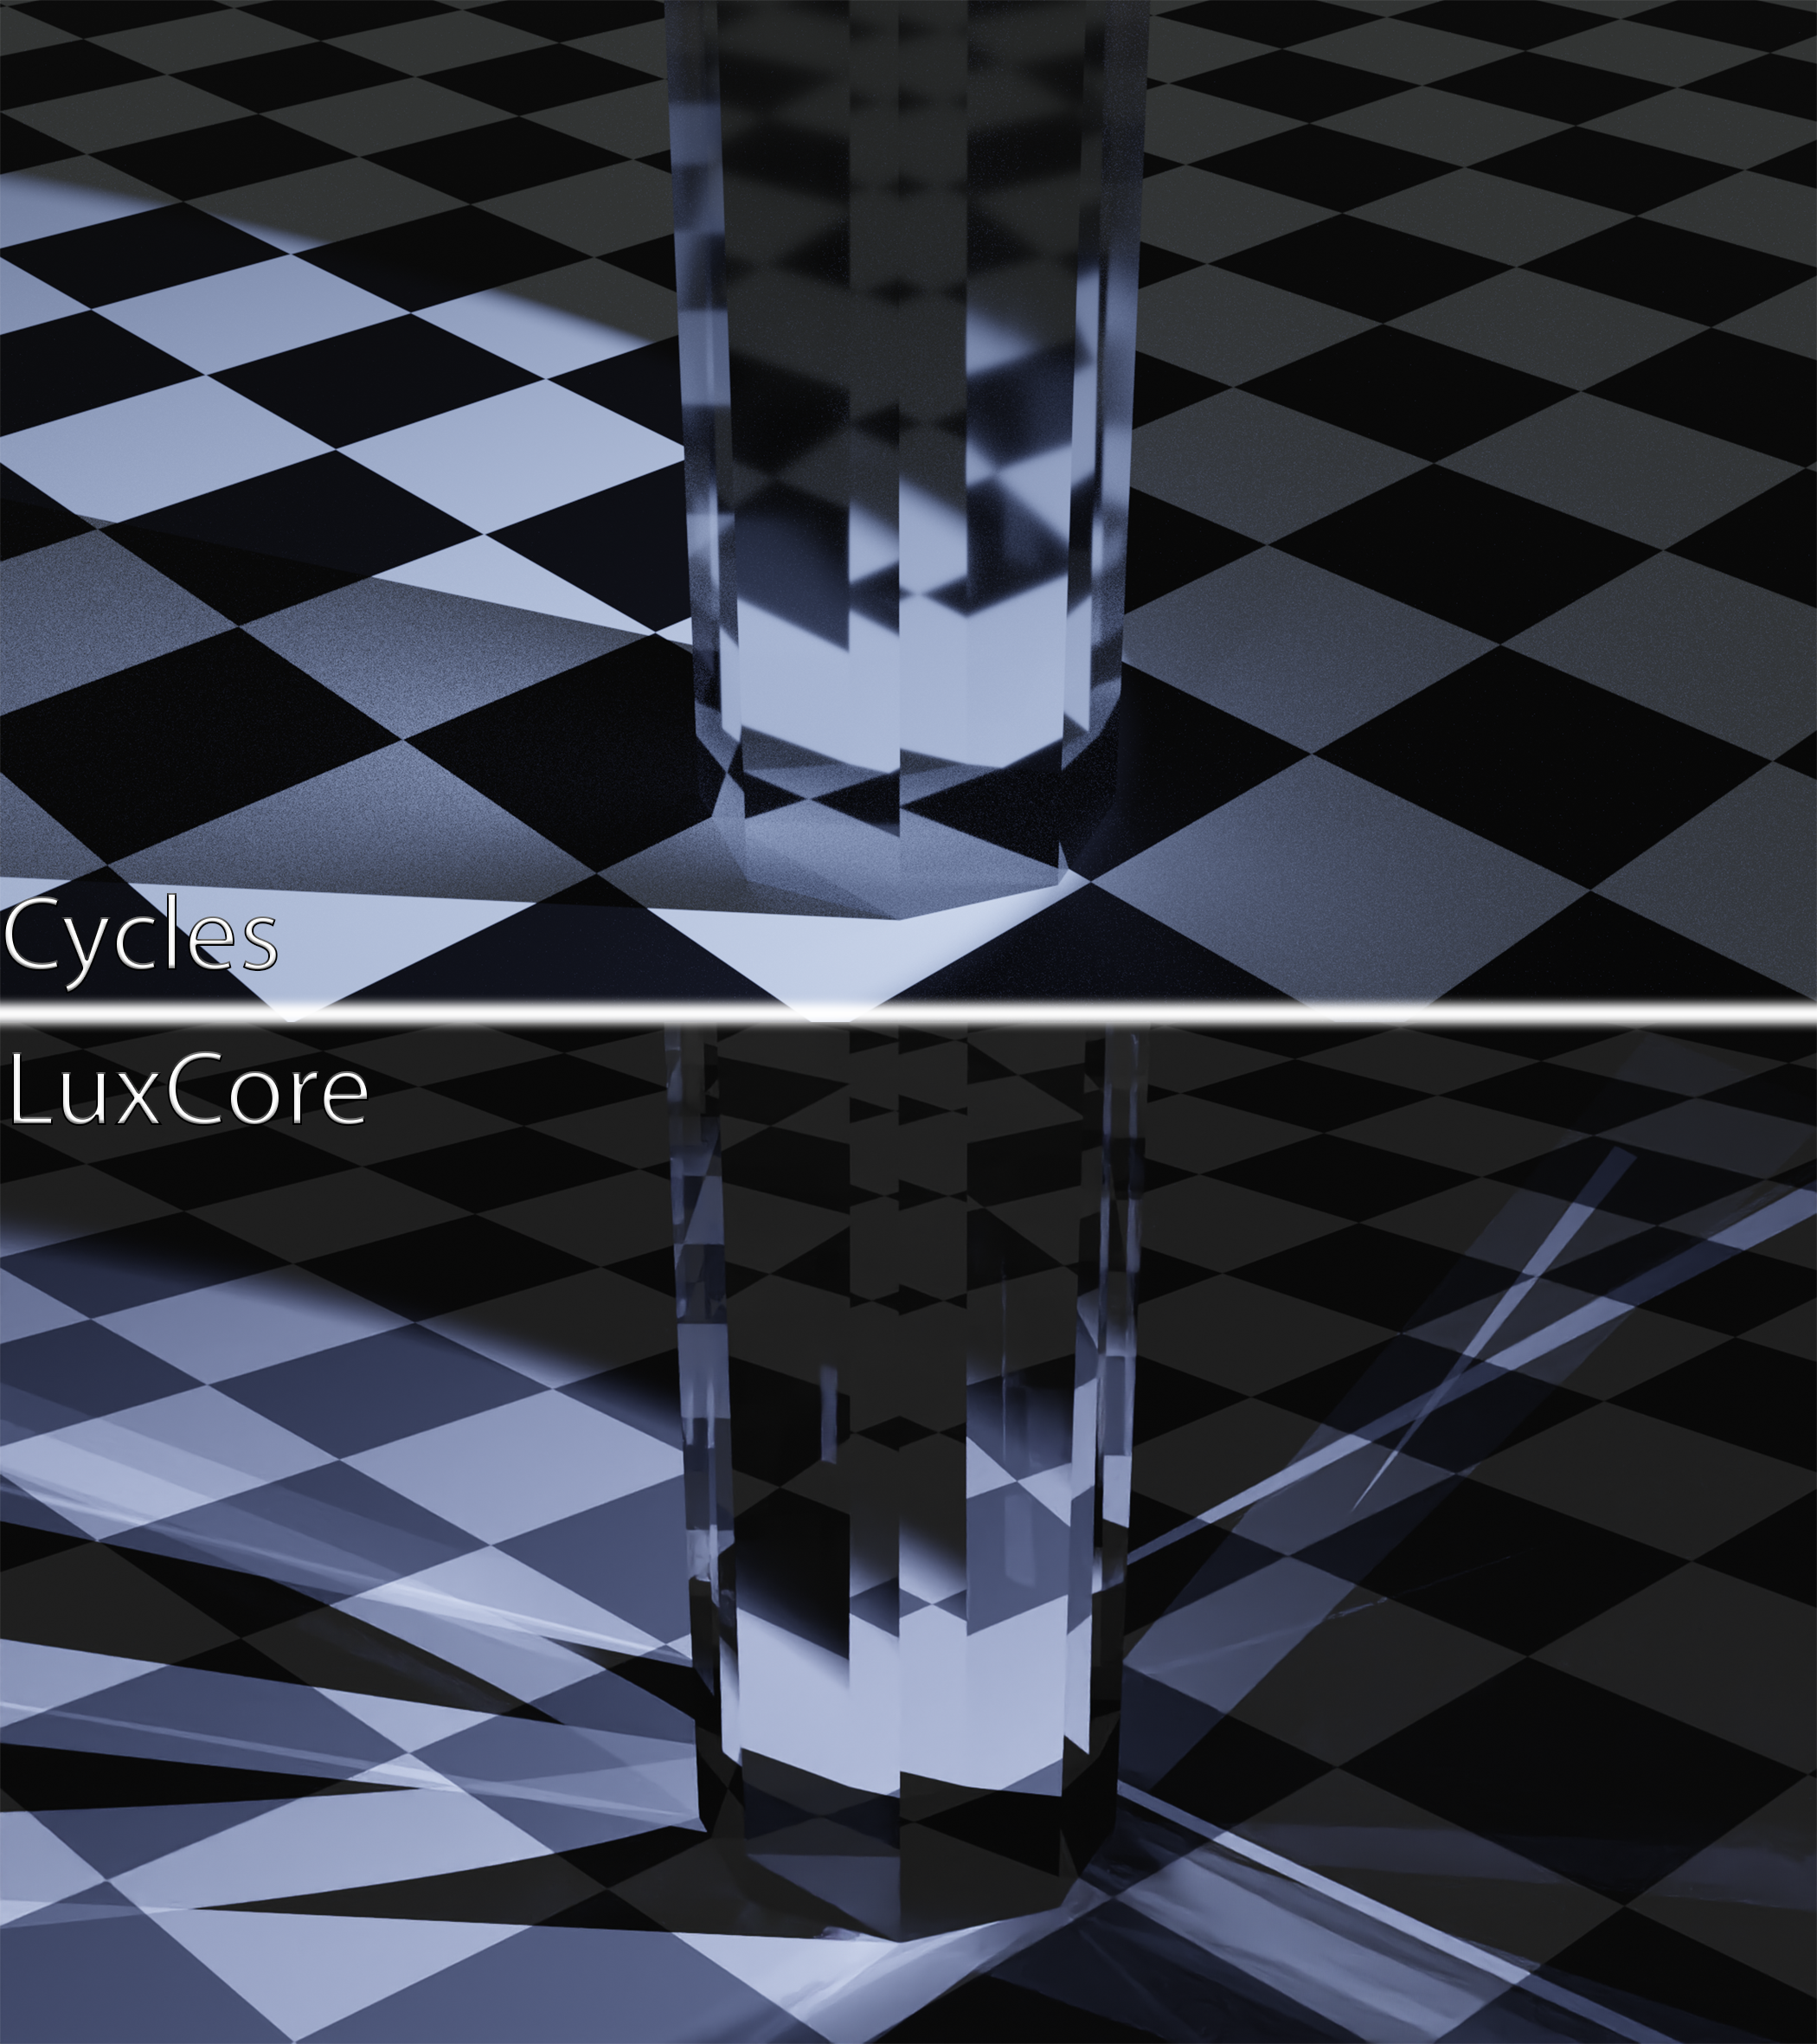
\includegraphics[scale=0.5]{Images/LuxVSCyclesOnGlass.png}
        
        \caption{Cycles vs LuxCore caustics}
        \label{fig:causticsCompare}
    \end{figure}
    
Cycles lack this feature, thus producing less than desirable results. This is because cycles tries to brute force it's way through the glass surface, but as a result most of the light rays reach their maximum number of bounces before exiting the object due to refraction. This causes the render to look nothing like it should with a real glass object, but if we increase the maximum number of bounces, it will introduce an artifact called "firefly" that appears as specs of white points on the screen. LuxCore has no issue with this scene, since bi-directional path tracing allows it to realistically recreate light paths being refracted by light and not waste computational power on rays that would never leave the object. LuxCore is also helped by it's powerful denoiser, allowing it to detect any fireflies that may appear, then removing them from the final image. 

\hfill
\subsection{Render times}
As evident by the data presented on tables \ref{table:cyclesTime} and \ref{table:luxTime}, GPU rendering is way more powerful compared to CPU solutions. This is because GPUs are specialised hardware focused on high complexity calculations that are perfect for this use case, rather than lots of small, simple operations like CPUs do.

\setlength{\arrayrulewidth}{0.3mm}
\begin{table}[h!]
\large
\begin{center}
\begin{tabular}{|c|c|c| } 
 \hline
  Cycles & BMW & ArchViz \\ 
  \hline
 \hline
 \rowcolor{red!15}AMD FX-4130 & 37:40 & 1:31:00 \\
 \hline
 \rowcolor{blue!15}Intel Core i5-7300HQ & 12:00 & 36:40 \\ 
 \hline
 \rowcolor{blue!15}Intel Core i5-6600 & 10:20 & 30:40 \\ 
 \hline
 \hline
 \rowcolor{green!15}Nvidia GeForce GTX 960 & 04:40 & 20:40\\
 \hline
 \rowcolor{green!15}Nvidia GeForce GTX 1050Ti & 04:20 & 18:20\\
 \hline
 \rowcolor{green!15}Nvidia GeForce GTX 1060 & 02:40 & 12:40\\
 \hline
 \hline
 \hline
  LuxCore & BMW & ArchViz \\ 
  \hline
 \hline
 \rowcolor{red!15}Nvidia GeForce GTX 960 & 12:40 & 28:40\\
 \hline
 \rowcolor{blue!15}Nvidia GeForce GTX 1050Ti & 09:00 & 23:00\\
 \hline
 \rowcolor{green!15}Nvidia GeForce GTX 1060 & 06:00 & 16:40\\
 \hline
\end{tabular}
\caption{Render times comparison}
\label{table:cyclesTime}
\end{center}
\end{table}

\section{Conclusion}
In this paper we pointed out the key differences between LuxCoreRender, Cycles and EEVEE both in rendering methods and results. We also tested them on different hardware to see if it is possible to use these engines on home configurations effectively.

\subsubsection{Hadware chioce}
    From the data provided above we can conclude that, yes, it is absolutely possible to use LuxCore, Cycles or EEVEE even for professional purposes. However let us not forget that rendering time will rise as the scene complexity goes up.
    
    We can also conclude that, on standard home computer configurations, CPU rendering is highly inefficient or even impossible on some older CPUs as we have seen it in the case of the FX-4130 LuxCore render (section \ref{cpu_rendering}). Also, newer CPUs usually feature an integrated graphic chip (As we see on the tested Intel CPUs, but the same case applies to the AMD Ryzen series).

    
    On low core-count systems GPU rendering is a much better choice, and it is probably a good idea to use a newer generation one. While higher-class GPUs are much more powerful this also means they need more power to operate not to mention the higher entry cost.

\subsubsection{Engine differences}
    First of all, we would like to make it clear, that these three engines are not better or worse compared to each other. Every one of them is for a different purpose. The main question of this paper is "What rendering engine should I use for my project?".
    
    As we have seen it, in production quality, for example advertisements, presentations, etc., where realism is key, it is good idea to use either LuxCore or Cycles and pre-render our scene. This results in much more photo realistic images. If light plays a crucial part in our scene LuxCore can be the best choice for us, as LuxCoreRender was designed to deal with complex light rays. (section \ref{luxCore}) However if our scene is much simpler (for example a product design) Cycles can save us a lot of time. (section \ref{cycles_section})
    
    EEVEE is best used only for real-time rendering. (section \ref{eevee_section}) For example in video games or 3D simulations where we need to see the results of our changes instantly. It is also worth mentioning that EEVEE is highly compatible with Cycles renderer. Because of this EEVEE can also be used to prototype a scene which will be rendered in Cycles at a later time.
    \newpage


\bibliographystyle{ieeetr}
\bibliography{References}

\end{document}